\chapter{Future Work and Conclusion}

summarize dissertation

new applications: storytelling + (ones in chapter 1)

\section{Known Issues}
In this section, we list some of the issues encountered in designing and building CueNet. Some of these are active areas of research, and whereas others are specific to our framework, and can be considered potential areas of research. Our experience with CueNet indicates that the following issues should be approached in a holistic manner, i.e., in conjunction with each other. Approaching these problems in the context of each other reduces the individual complexity of each sub-problem by possibly increasing the complexity of the entire framework, but making the problem more tractable.

\textbf{\textbf{Noise in Social Media}}: The problem of noise filtering in web data is a prominent one, and is being addressed by various communities in different ways. These range from entity matching and record linkage problems \cite{elmagarmid2007duplicate} to correcting missing data in information networks \cite{sadikov2011correcting}. These problems get trickier because of the different variations in representing tiny details such as representation names of people, addresses of places, and time. In fact, there is a whole school of anthroponomastics \cite{schneider2009s} dedicated to studying variations in human names. Ideas in this field indicate that these differences arise due to cultural, historical and environmental issues\cite{al2009socio}. Such issues cannot be trivially addressed. 

%Consider, for example, the Hebrew name below:
%
%\begin{figure}[h]
%\centering
%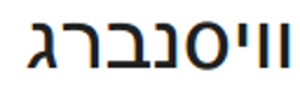
\includegraphics[width=0.15\textwidth]{media/ronen.png}
%\label{fig:exp-general-loc-cx}
%\end{figure}
%
%It can be translated to English as ``Waisenberg" or ``Vaisenberg". So are Mr.\ X Waisenberg who authored a paper in a Security conference and Dr.\ X Vaisenberg who works at Google, the same person? They might be if X has semitic origins!

Face tagging in social media sources like Facebook can also be very noisy. This strictly prohibits directly using this data to train verification/recognition models. Also, the quality of photos are poor, resulting in weaker features, which would have otherwise allowed better matching. 

An exhaustive scientific characterization of noise in social media is beyond the scope of this paper, and is being investigated step by step in social media research communities.

\textbf{\textbf{CPU Efficiency}}: The query engine in CueNet is responsible for extracting data from different sources. If a very large number of photos are being tagged, our scheme of query generation and merging will prove inefficient. Processing many photos from different people provides a very rich opportunity to develop interesting heuristics using event semantics for the multi-query optimization problem. Also, partitioning the discovery algorithm such that the computations can occur in a distributed manner is a complex problem. Such steps will be required if the application workload is of the scales of Facebook or processing photos in real time at the scales of Instagram.

\textbf{\textbf{Face Verification}}: Even though face recognition has been studied in research for the last two decades, face verification, and its specific application to faces in the wild has been a relatively recent venture. Although the accuracy of these systems is commendable, the problems of occlusion, image quality, face alignment and differing lighting conditions exist. These hard problems need to be solved before ``perfect" or ``near-perfect" verification can be established. 

\textbf{\textbf{Execution Patterns}}: When is a good time to execute the algorithm? When a user takes a photo? Or before she uploads it to her favorite photo sharing site? For the current evaluation, contextual sources are assumed to be immutable. This is not true in the real world. Contextual sources are constantly being appended with new information, and old information is being updated. These updates may be vital in tagging a certain photo. So the question of when to execute the algorithm, or how and when to query the sources is an open question. If a large number of photos are to be tagged, and a busy source like Facebook is being used for context, the CueNet query engine must take into account various freshness metrics and crawling policies of the sources. 

\textbf{\textbf{Open Datasets}}: The unavailability of a large public data set over which different techniques can be evaluated against each other is an open problem. As seen in our experiments, personal information is vital to contextual approaches, and this data is largely personal, and therefore cannot be shared openly. Optimal anonymization techniques need be to invented such that the privacy of the experiment participants are maintained, and at the same time the data is meaningful to be applied in contextual approaches to problems. This need to be solved so that new context discovery techniques can be evaluated independently and against each other, over a common platform.


Problems/Opportunities:

  1. Absence of a language/tool which can be used to express real world models. Ontologies are logic driven. Usually deal with true/false.

  2. Starting points of such a language -- physical variables, graphics world modeling, entity identification.

  3. Backtracking based algorithms.
